\documentclass{standalone}
\usepackage{tikz}
\usetikzlibrary{decorations.pathreplacing}
\begin{document}

            % TIKZ
            %$\left\{
                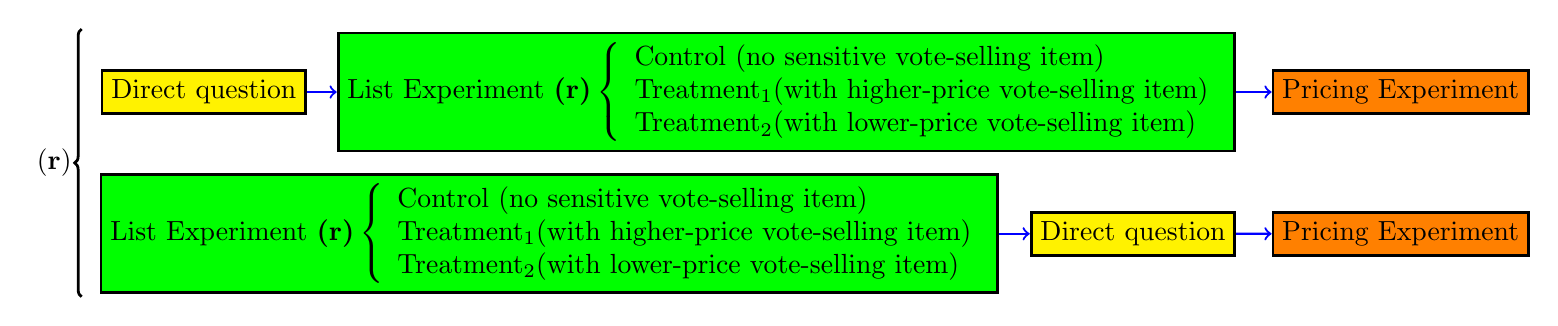
\begin{tikzpicture}[
                %scale=2
                scale=.2,
                line width=1pt] %

% random
\draw[decoration={brace,mirror,raise=10pt},decorate]
  (-28,-2) -- node[black,midway,xshift=-0.7cm] {({\bf r})} (-28,-19);

                    % 1
                    \node[draw,align=center,fill=yellow,text=black] (ArgumentA1) at (-22,-6) {Direct question}; % 1
                    \node[draw,align=center,fill=green,text=black] (ArgumentB1) at (15,-6)   {List Experiment  % 2
                    $
                  \mbox{{\bf (r)}}
                  \left\{
                        \begin{array}{llc}
                            \mbox{Control (no sensitive vote-selling item)}\\
                            \mbox{Treatment}_{1} \mbox{(with higher-price vote-selling item)}\\
                            \mbox{Treatment}_{2} \mbox{(with lower-price vote-selling item)}\\
                          \end{array}
                    \right.
                    $};
                    %\node[draw,align=center, fill=red] (ArgumentC) at (60,-6) {Conjoint experiment}; % 3


                    %\draw[->,draw=blue,thick] (ArgumentB1) to (ArgumentC);
                    \draw[->,draw=blue,thick] (ArgumentA1) to (ArgumentB1);


                    %\node at (6., -1.-6) {};



                    % 2
                    \node[draw,align=center,fill=green,text=black] (ArgumentA2) at (-.05,-15) {List Experiment  % 1
                    $
                    \mbox{{\bf (r)}}
                    \left\{
                        \begin{array}{llc}
                            \mbox{Control (no sensitive vote-selling item)}\\
                            \mbox{Treatment}_{1} \mbox{(with higher-price vote-selling item)}\\
                            \mbox{Treatment}_{2} \mbox{(with lower-price vote-selling item)}\\
                          \end{array}
                    \right.
                    $};
                    \node[draw,align=center,fill=yellow,text=black] (ArgumentB2) at (37,-15) {Direct question}; % 2
                    %\node[draw,align=center, fill=red] (ArgumentC) at (60,-15) {Conjoint experiment}; % 3





                    %\draw[->,draw=blue,thick] (ArgumentB2) to (ArgumentC);
                    \draw[->,draw=blue,thick] (ArgumentA2) to (ArgumentB2);



 % Pricing Experiment arriba 
                    \node[draw,align=center,fill=orange,text=black] (ArgumentC1) at (54,-6) {Pricing Experiment}; % 1
                    \draw[->,draw=blue,thick] (ArgumentB1) to (ArgumentC1);


 % Pricing Experiment abajo
                    \node[draw,align=center,fill=orange,text=black] (ArgumentC2) at (54,-15) {Pricing Experiment}; % 1
                    \draw[->,draw=blue,thick] (ArgumentB2) to (ArgumentC2);


                    \end{tikzpicture}
               % \right.$

\end{document}